%%%%%% CMB-S4 Simulations and Data Analysis Chapter  %%%%%%%%%%%%%%%%
 
\chapter{Simulations and Data Analysis}
%\renewcommand*\thesection{\arabic{section}}

%%%%%%%%%%%%%%%%%%%%%%%%%%%%%%%%%%%%%%%%%%%%%%%%%%%%%%%%%%%
%%%%%%%%%%%%%%%%%%%%%%%%%%%%%%%%%%%%%%%%%%%%%%%%%%%%%%%%%%%
%%%%%%%%%%%%%%%%%%%%%%%%%%%%%%%%%%%%%%%%%%%%%%%%%%%%%%%%%%%
%%%%%%%%%%%%%%%%%%%%%%%%%%%%%%%%%%%%%%%%%%%%%%%%%%%%%%%%%%%

\section{Introduction}

Extracting science from a CMB dataset is a complex, iterative process requiring expertise in both physical and computational sciences. In this chapter we start with an overview of the data analysis pipeline before diving more deeply into its subsets - time-orderd data processing, component separation and the estimation of statistics and parameters. We then discuss the drivers for, and corresponding structure of, the simulation pipeline, and describe in detail its sky modeling and data simulation subsets. Finally we assemble the full simulation and data analysis pipeline, noting its inherently iterative structure, and discuss its critical uses in forecasting and validation and verification, before concluding with a discussion of some key implementation issues. Throughout our goal is to describe the current state of the art, note the particular challenges posed by CMB-S4, and describe how they might be addressed.

\section{Data Analysis Overview}

\begin{figure}[htbp]
\begin{minipage}[h]{0.7\linewidth}
The reduction of a CMB data set typically proceeds in a sequence of steps:
\begin{description}
\item[ Pre-processing:] The raw time-ordered detector data are calibrated and gross time-domain systematics are either removed (typically by template subtraction, filtering or marginalization) or flagged. The goal here is to make the real data match a model that will underpin all subsequent analyses.
\item[Map-making:] At each observing frequency, estimates of the intensity I and the Stokes Q- and U-polarizations of the sky signal are extracted from the cleaned time-ordered data based on their spatial stationarity, typically using some degree of knowledge of the instrument's noise properties.
\item[Component separation:] If sufficient frequenciy maps are available, the CMB can be separated from the various foreground sky components based on its unique spectral invariance (in CMB units).
\item[Power spectrum estimation:] The six auto- and cross-angular power spectra of the CMB temperature T and E- and B-mode polarizations are estimated from the CMB and/or frequency maps, and corrected for E- to B-mode lensing.
\item[Parameter estimation:] The best-fit parameters for any cosmological model are derived by comparing the theoretical TT, TE, EE and BB CMB power spectra that they would induce with the data and their uncertainties.
\end{description}
\end{minipage}
\begin{minipage}[h]{0.275\linewidth}
\centering
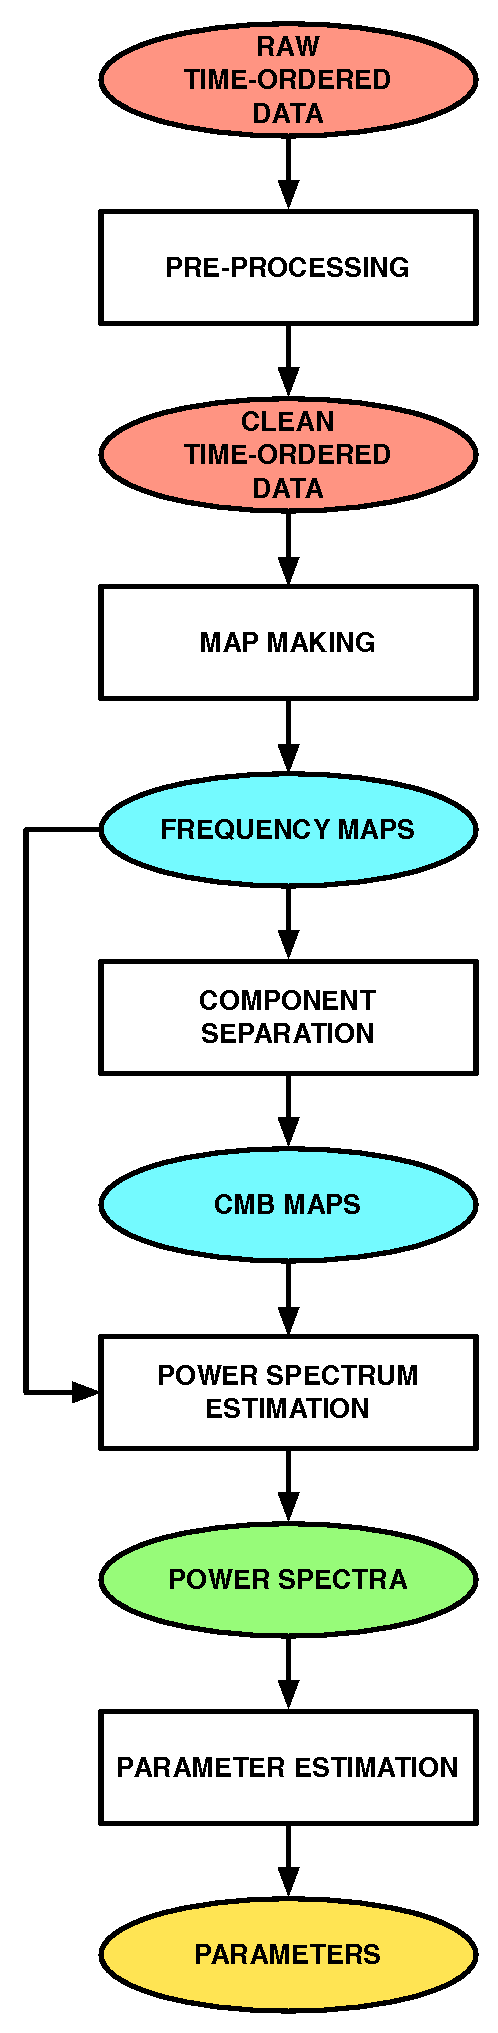
\includegraphics[width=0.5\textwidth]{Analysis/dr}
\caption{CMB data reduction}
\label{fig_dr}
\end{minipage}
\end{figure}

This reduction essentially consists of a series of changes of basis for the data, from time samples (red) to map pixels (blue) to spectral multipoles (green) to cosmological parameters (yellow), with each basis-change reducing the data volume, increasing the signal-to-noise, and exposing a different class of systematic effects for mitigation.

Note however that the data can only remain a sufficient statistic at each step in the reduction if we also propagate its full covariance matrix. Since this is an ${\cal N}_b \times {\cal N}_b$ matrix in the dimension of the basis, its construction, manipulation and reduction pose the greatest computational challenge to this analysis. In particular the full pixel-domain data covariance matrix is generally dense and unstructured, requiring O(${\cal N}_p^3$) operations to build and O(${\cal N}_p^2$) bytes to store. All the major drivers of CMB science - polarization sensitivity, higher resolution, larger sky coverage - push us towards larger pixel counts, with an instrument mapping a fraction of the sky $f_{sky}$ with a beam of $b$ arcminutes covering O($10^9 \, f_{sky}/b^2$) pixels per IQU-component. For the last decade or more the computational intractability of the resulting pixel-domain matrices has forced us to replace explicit covariance propagation with Monte Carlo methods in all but a limited set of small sky fraction/low resolution cases.

\begin{figure}[htbp]
\centering
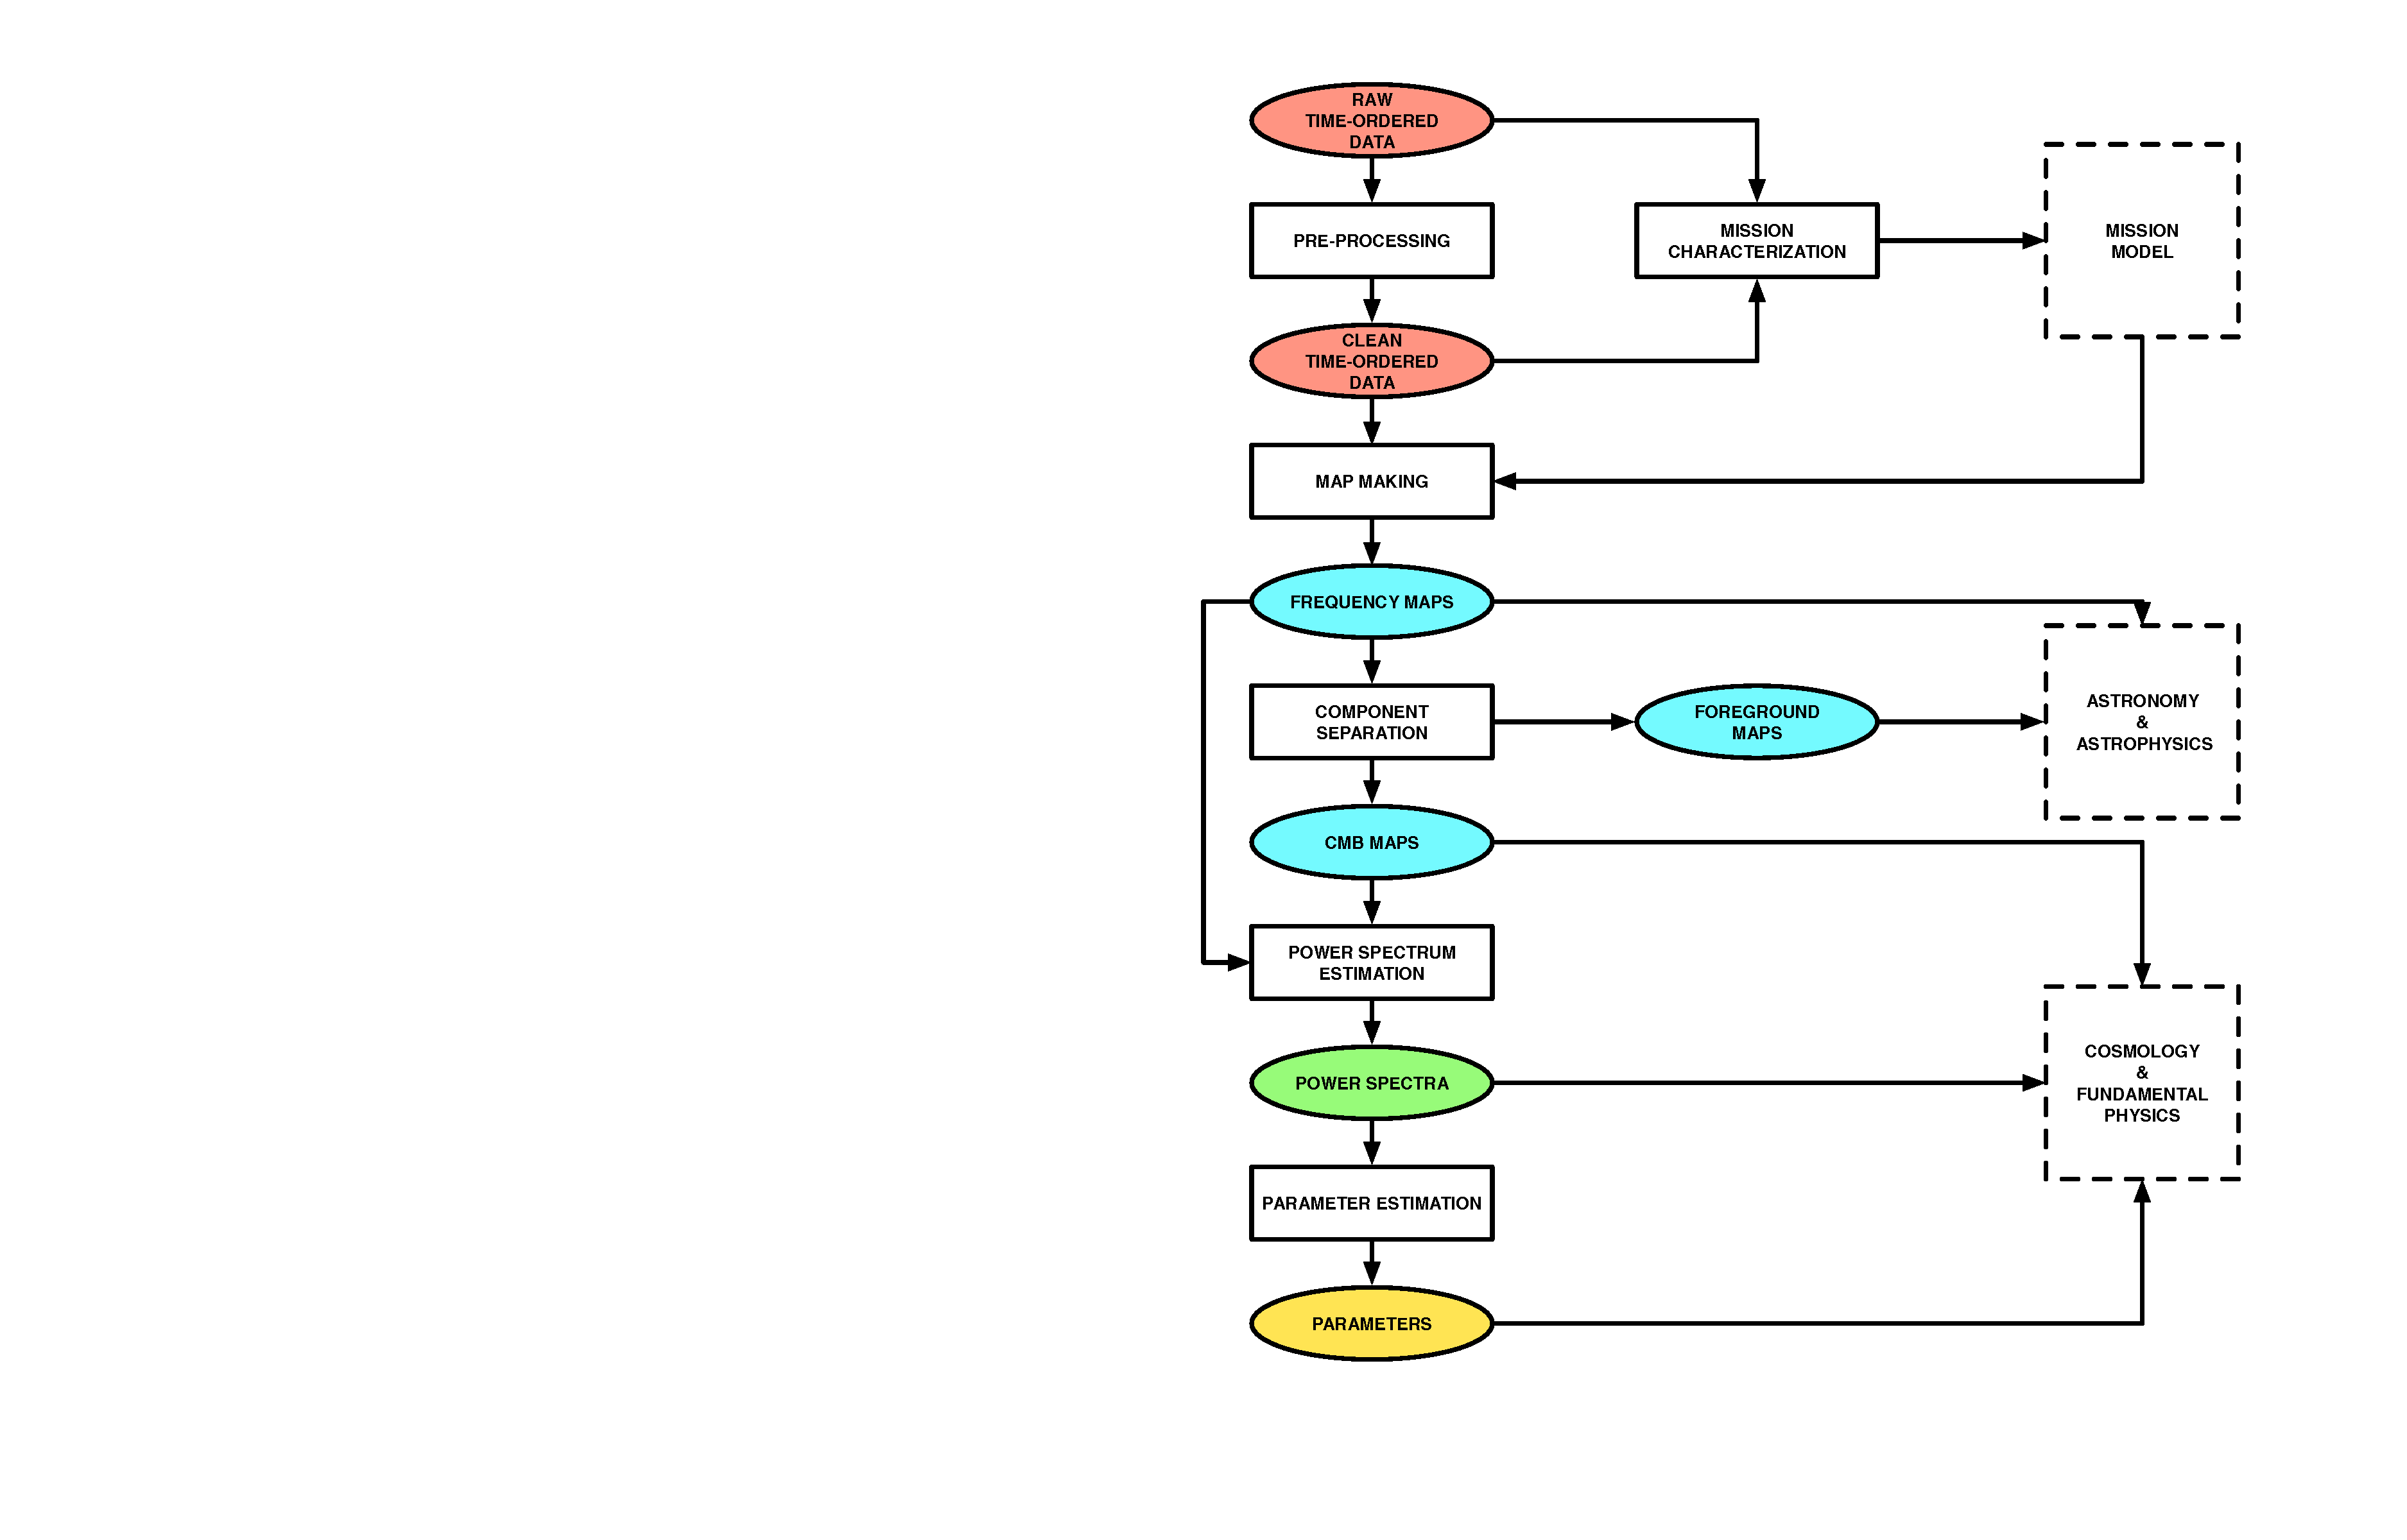
\includegraphics[width=1\textwidth]{Analysis/da}
\caption{The CMB data analysis pipeline}
\label{fig_da}
\end{figure}

Beyond this basic data reduction, the full analysis pipeline (Figure \ref{fig_da}) also includes mission characterization and science exploitation branches. Time domain data are extensively used to build a model of the mission, comprising the instrument and the observation. For the instrument this modeling can include such steps as determining beam profiles and estimating noise properties (including cross-correlations); for the observation, it includes reconstructing the detector pointing and polarization orientation from telescope sensor data, and incorporating atmosphere records in the data-flagging. The resulting mission model then feeds back into all of the ensuing data reduction and interpretation. The primary science exploitation derives cosmology and fundamental physics results from the various correlation functions of the CMB maps, from the power spectra's energy scale of inflation and neutrino mass to the higher-order statistics'  measures of non-Gaussianity and the lensing potential. In addition the frequency maps represent important astronomical and astrophysical observations, particularly when the frequency sampling is sufficient to isolate individual foreground components along with the CMB. 

\newpage

\input Analysis/tod_processing.tex

\newpage

\input Analysis/component_separation.tex

\newpage

\input Analysis/statistics_parameters.tex

\newpage

\section{Simulation Overview}
Simulations of a CMB mission's data play a number of critical roles; specifically they are required for
\begin{itemize}
\item Forecasting: informing the design and development of a mission to ensure that it is capable of meeting its science goals.
\item Validation and verification: ensuring that all of our data analysis tools meet their requirements and specifications.
\item Uncertainty quantification and debiasing: providing an alternative to the full data covariance matrix when this is computationally intractable.
\end{itemize}

As shown in Figure \ref{fig_sim}, given a mission model (both instrument and observation) and a sky model (both CMB and extra-galactic and galactic foregrounds) we can generate a simulation of the mission data in any of its domains. However, there is an inevitable trade-off between how representative the simulation is of real data and the complexity of the input models and computational cost of generating the simulation. The choice of the simulation data domain will then be determined by the balance between the realism requirements and the complexity/cost constraints for the particular task at hand.

\begin{figure}[htbp]
\centering
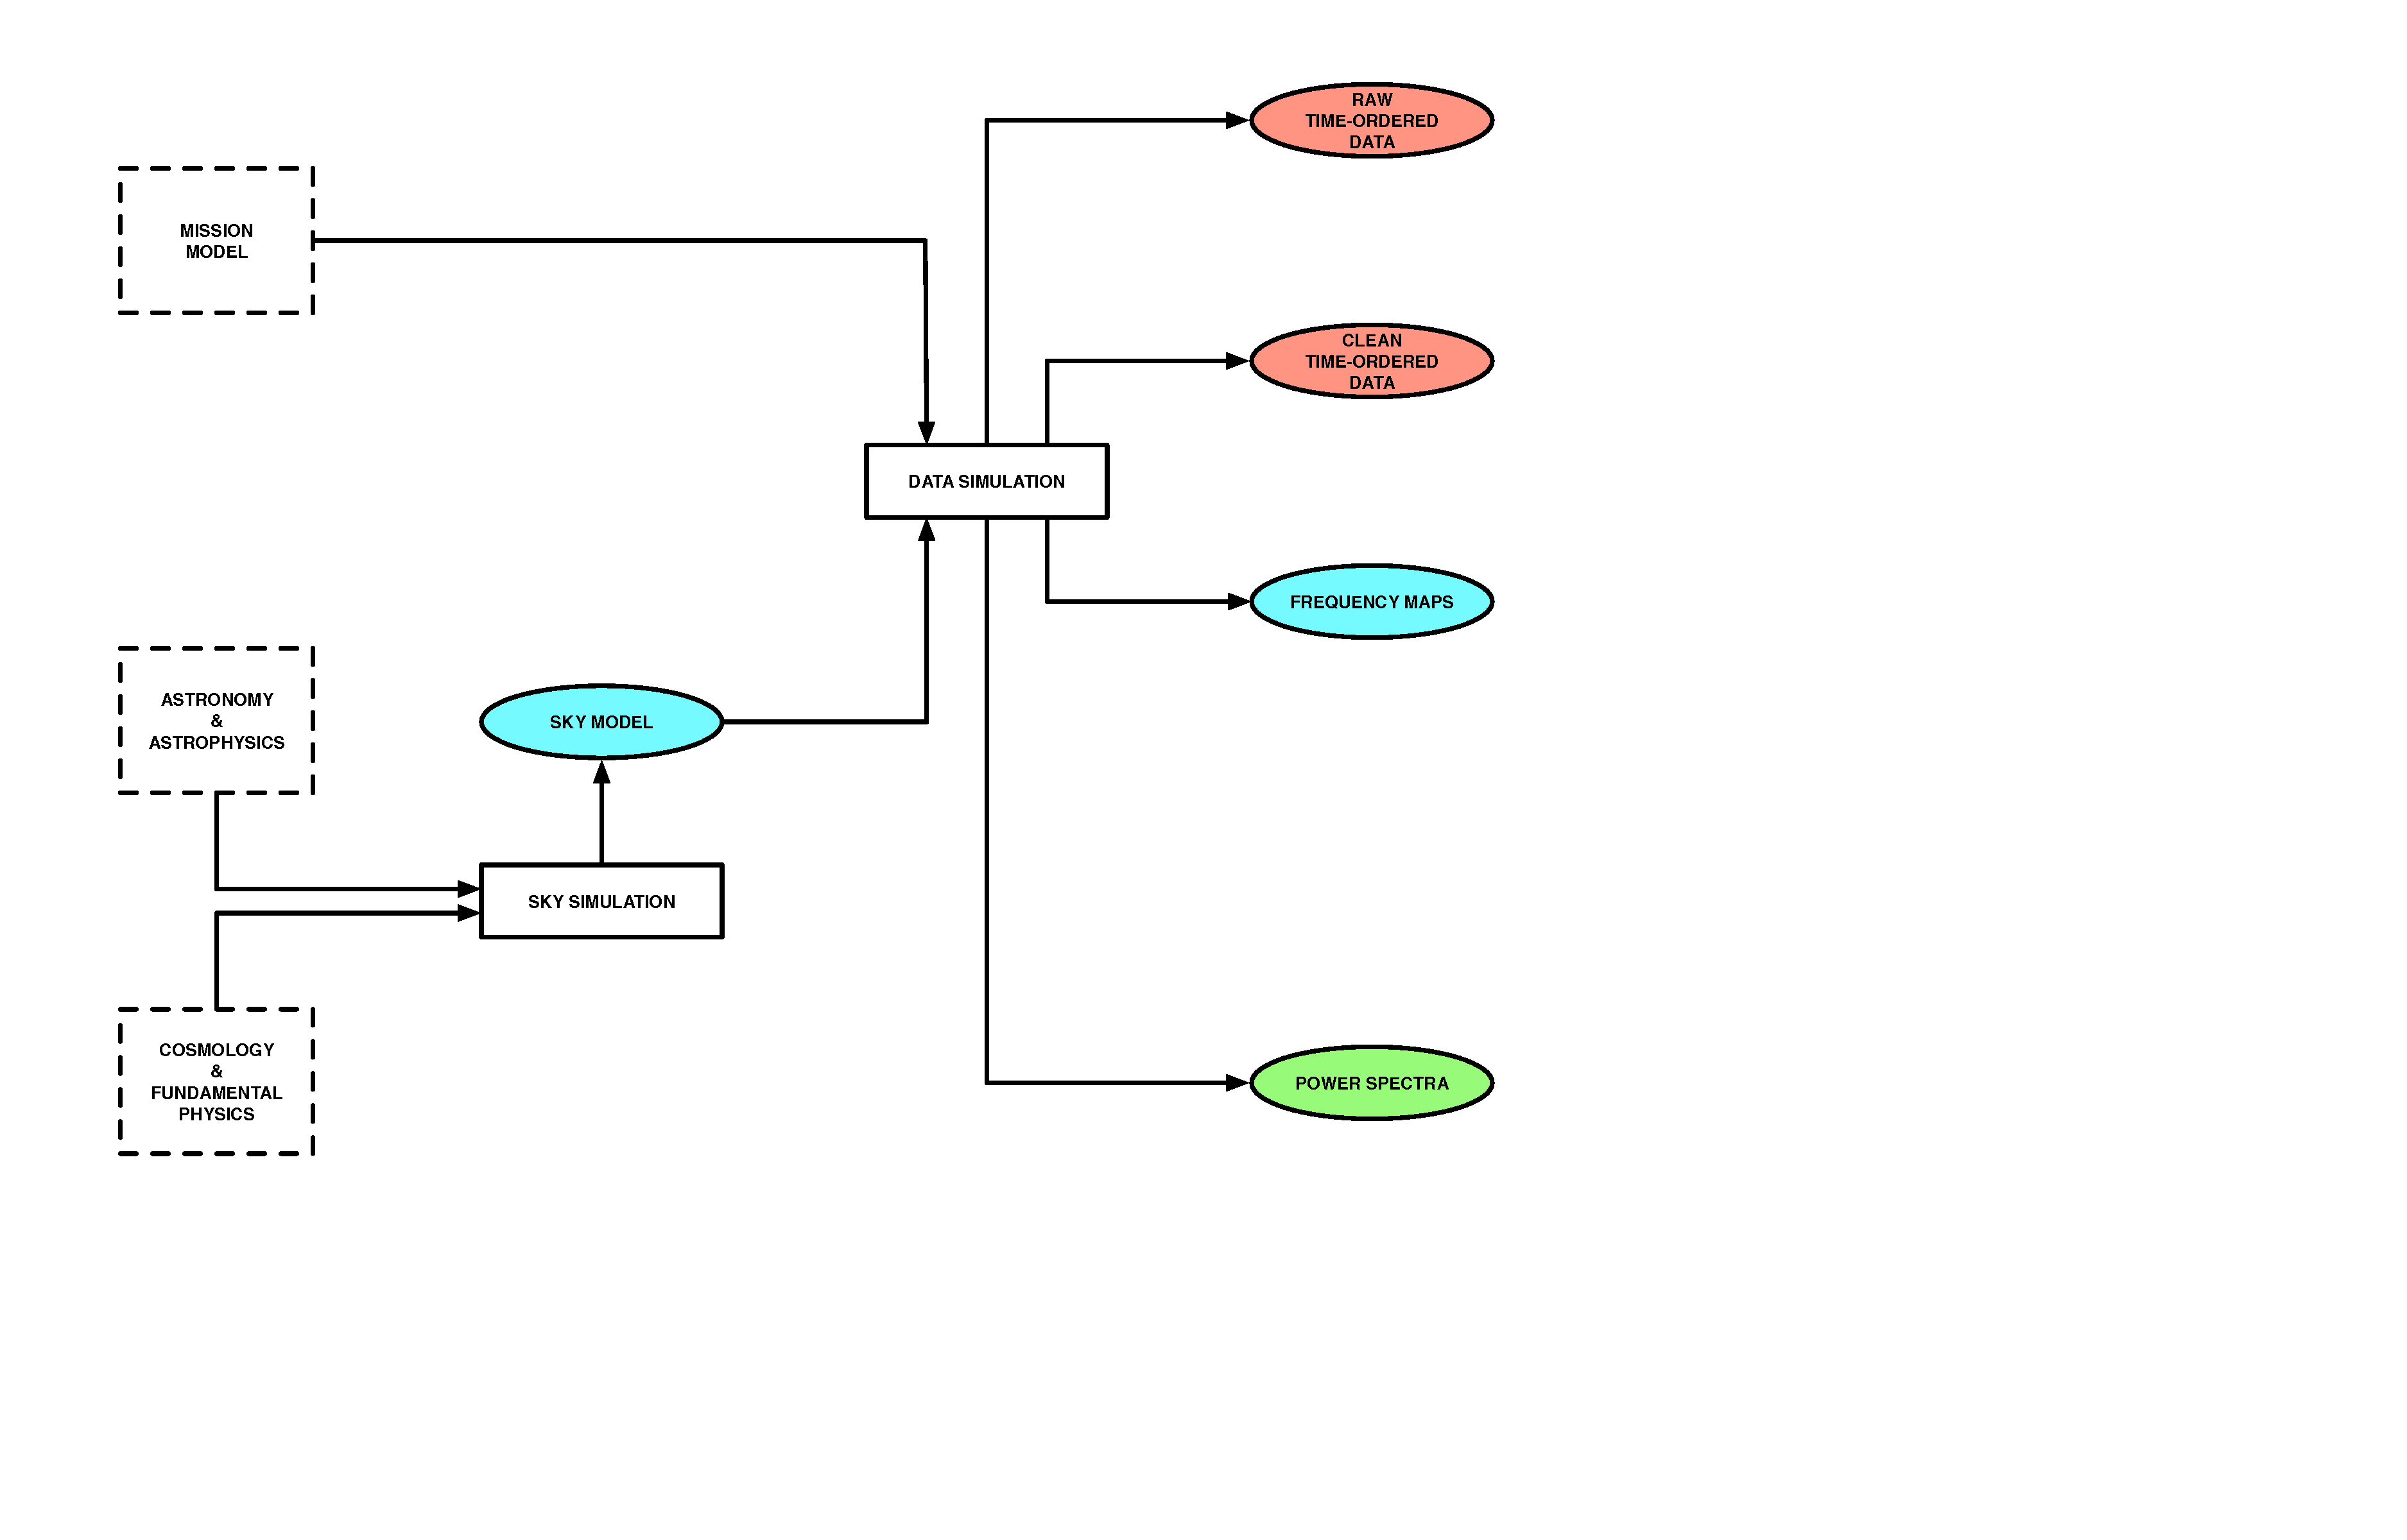
\includegraphics[width=1\textwidth]{Analysis/sim}
\caption{The CMB simulation pipeline}
\label{fig_sim}
\end{figure}

The generation of the input mission and sky models are themselves far from trivial tasks. The mission model is typically derived from pre-deployment measurements of the instrument properties refined by characterization from the data themselves, together with ancilliary telescope and environmental data characterizing the observation; the sky model requires its own dedicated simulation capability which - since it is independent of the details of any single mission - can be a community-wide endeavor.

\newpage

\input Analysis/sky_modeling.tex

\newpage

\input Analysis/data_simulation.tex

\newpage

\section{The Simulation and Data Analysis Pipeline}

The overall simulation and data analysis pipeline (Figure \ref{fig_simda}) can now be seen as both a top-down data reduction process and a wrap-around refinement of our mission and sky modeling. Typically the two phases are interleaved, with each new data reduction improving our mission and sky models, which are in turn fed back into an improved data reduction.

\begin{figure}[htbp]
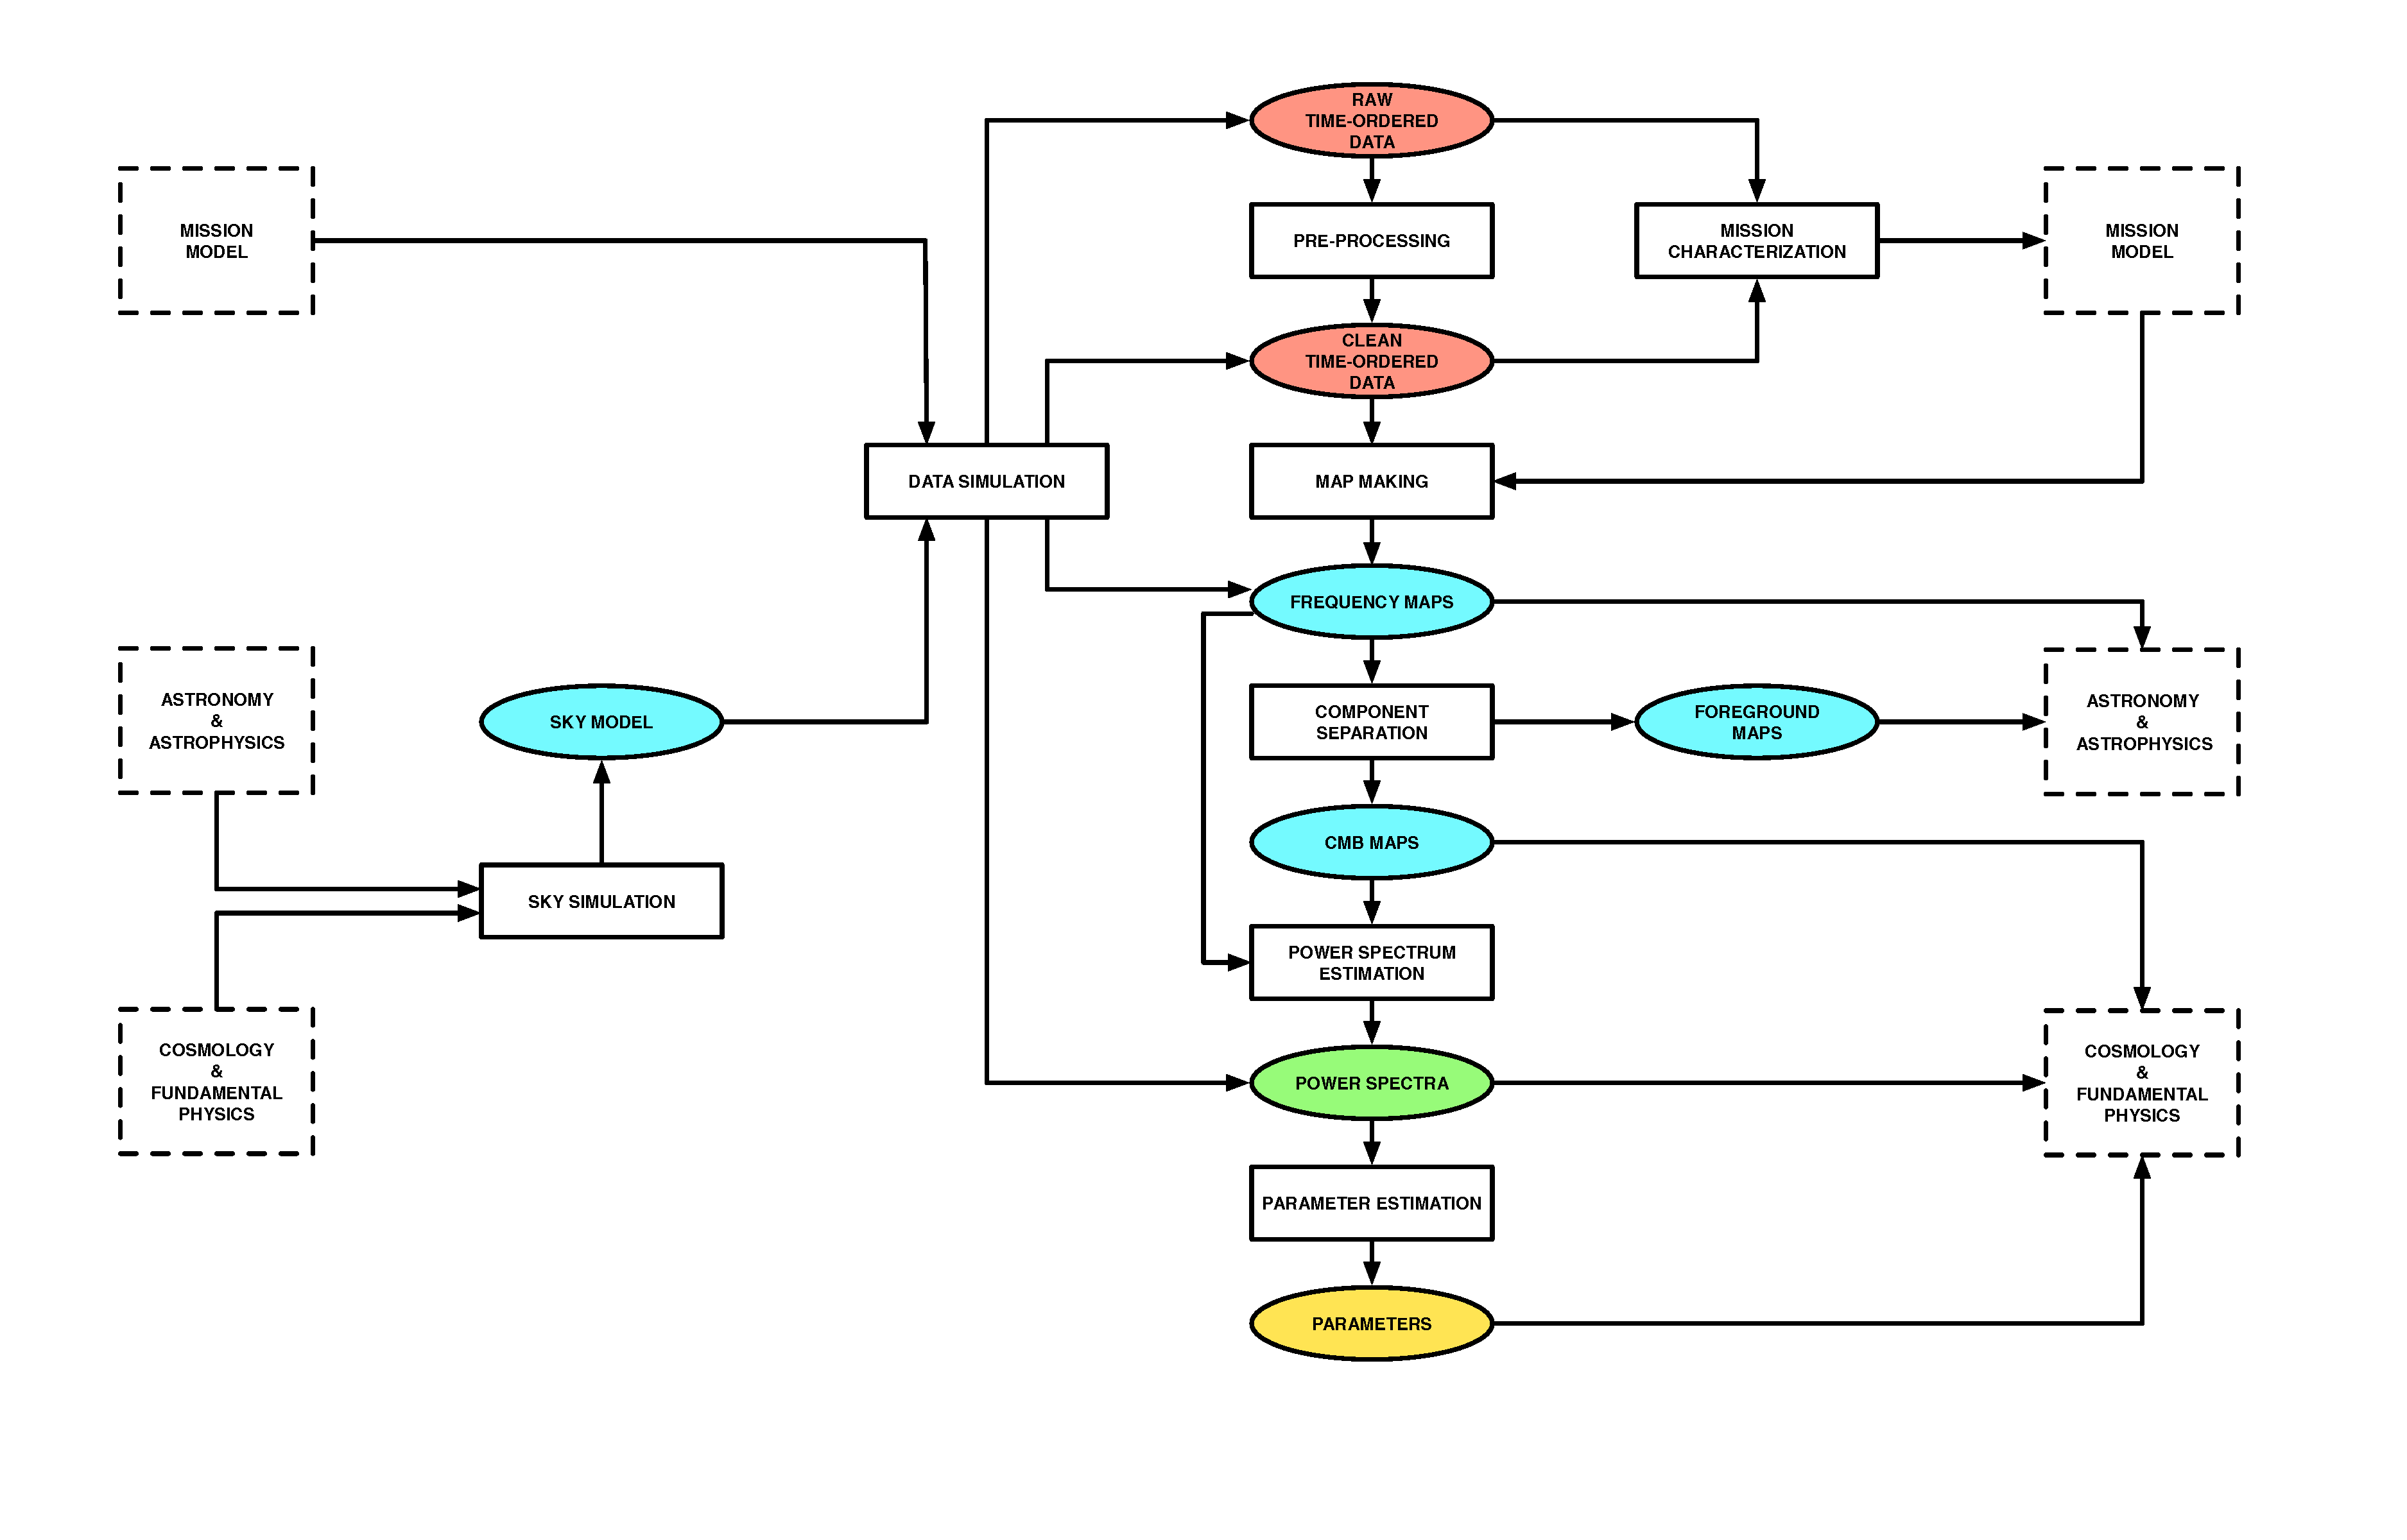
\includegraphics[width=1\textwidth]{Analysis/simda}
\caption{The full CMB simulation and data analysis pipeline}
\label{fig_simda}
\end{figure}

For CMB-S4 the most critical uses of this pipeline (or subsets thereof) are currently in forecasting and validation and verification. Further, the very discussion of such a pipeline provides a natural context in which to consider important implementation issues.

\newpage

\input Analysis/forecasting.tex

\newpage

\input Analysis/validation_verification.tex

\newpage

\input Analysis/implementation.tex


%\bibliography{cmbs4}

%%
%% Populate the .bib file with entries from SPIRES Bibtex (preferred)
%% or ADS Bibtex (if no SPIRES entry).
%%  SPIRES will also supply the CITATION line information; please include it.
%%


